\begin{frame}{Review}
  \begin{block}{Sensors, Features, and Machine Learning for Oil Spill Detection and Monitoring: A Review \cite{rs12203338}}
    \textit{Remote sensing technologies and machine learning (ML) algorithms play an increasingly   important role in accurate detection and monitoring of oil spill slicks, assisting scientists in forecasting their trajectories, developing clean-up plans, taking timely and urgent actions, and applying effective treatments to contain and alleviate adverse effects. Review and analysis of different sources of remotely sensed data and various components of ML classification systems for oil spill detection and monitoring are presented in this study. More than 100 publications in the field of oil spill remote sensing, published in the past 10 years, are reviewed in this paper.}
  \end{block}  
\end{frame}

\begin{frame}{Marco de trabajo - características}
  \footnotesize
  Marco general de trabajo
  \begin{figure}
      \centering
      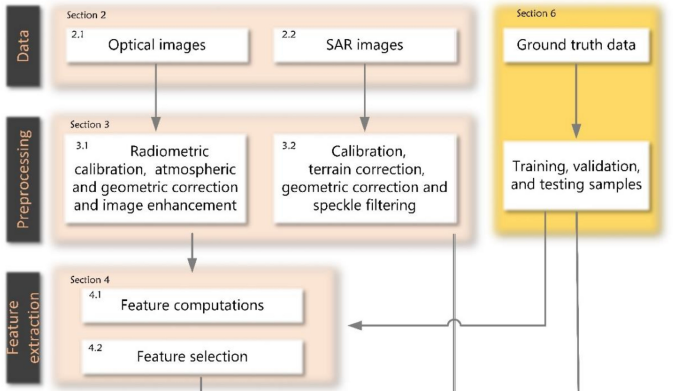
\includegraphics[scale=0.6]{img/section_02/framework_spill_detection.png}
      \caption{Preprocesamiento y extracción de características \cite{rs12203338}}
      \label{fig:preprocessing_and_feature_extraction}
  \end{figure}
\end{frame}

\begin{frame}{Marco de trabajo - algoritmos}
  \begin{figure}
      \centering
      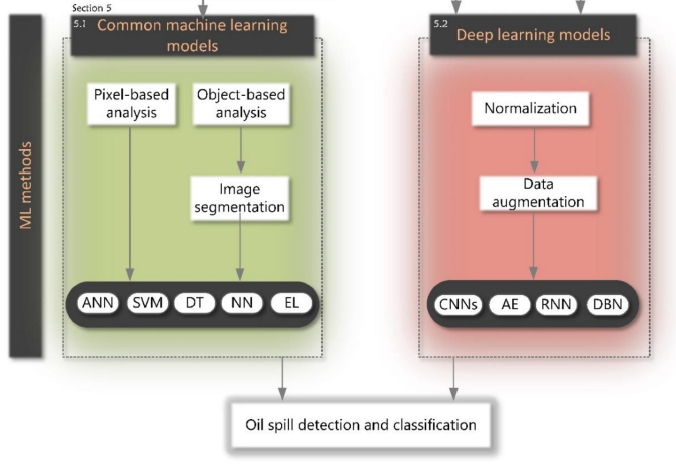
\includegraphics[scale=0.6]{img/section_02/framework_spill_detection2.png}
      \caption{Algoritmos de detección y clasificación \cite{rs12203338}}
      \label{fig:my_label}
  \end{figure}
\end{frame}

\begin{frame}{Imágenes ópticas}
  \begin{figure}
      \centering
      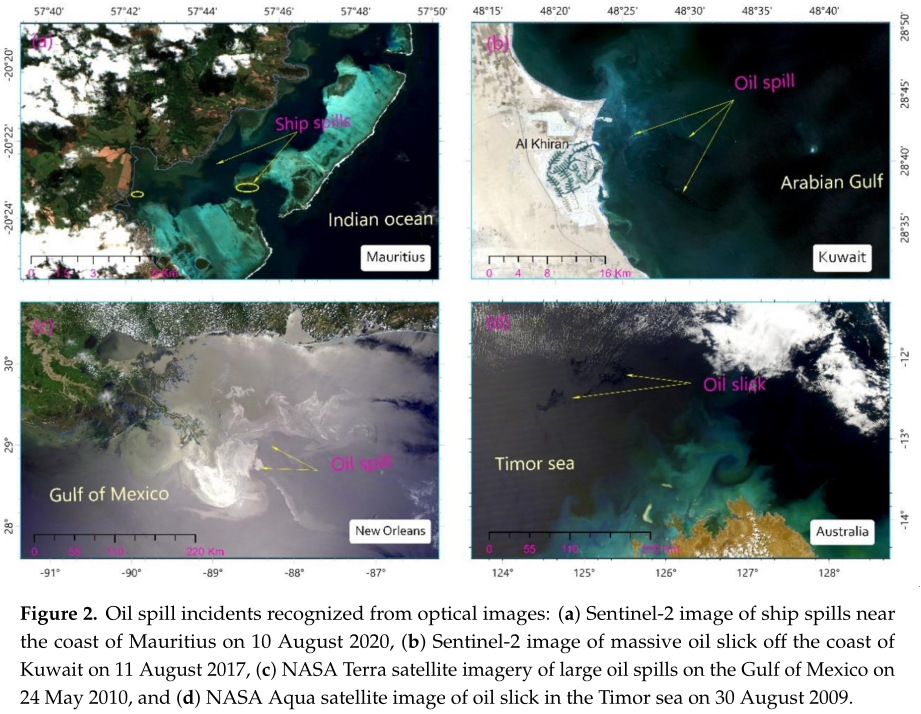
\includegraphics[scale=1.2]{img/section_02/caracteristicas_opticas_01.png}
      \caption{Imágenes multiespectrales}
      \label{fig:optical_features_01}
  \end{figure}
\end{frame}

\begin{frame}{Satélites ópticos}
  \begin{figure}
      \centering
      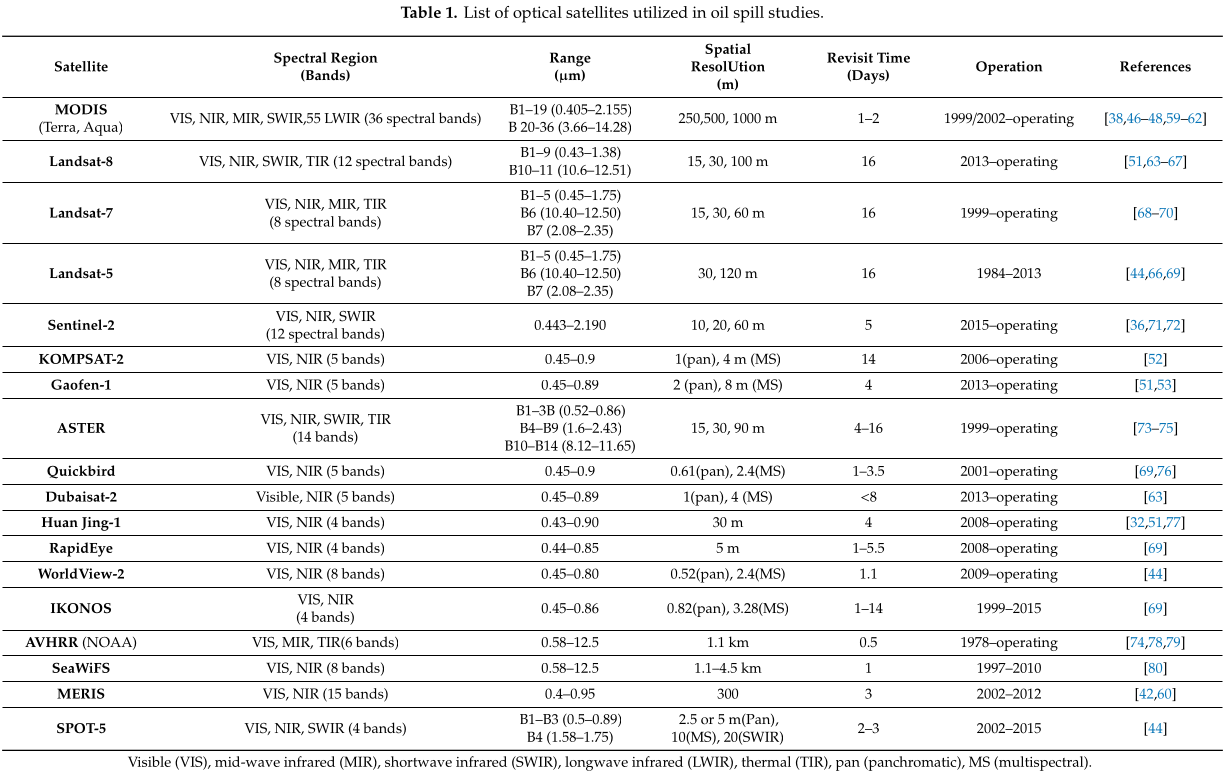
\includegraphics[scale=1.0]{img/section_02/caracteristicas_opticas_02.png}
      \caption{Lista de satélites multiespectrales e hiperespectrales usados}
      \label{fig:optical_features_02}
  \end{figure}
\end{frame}

\begin{frame}{Imágenes radar}
  \begin{figure}
      \centering
      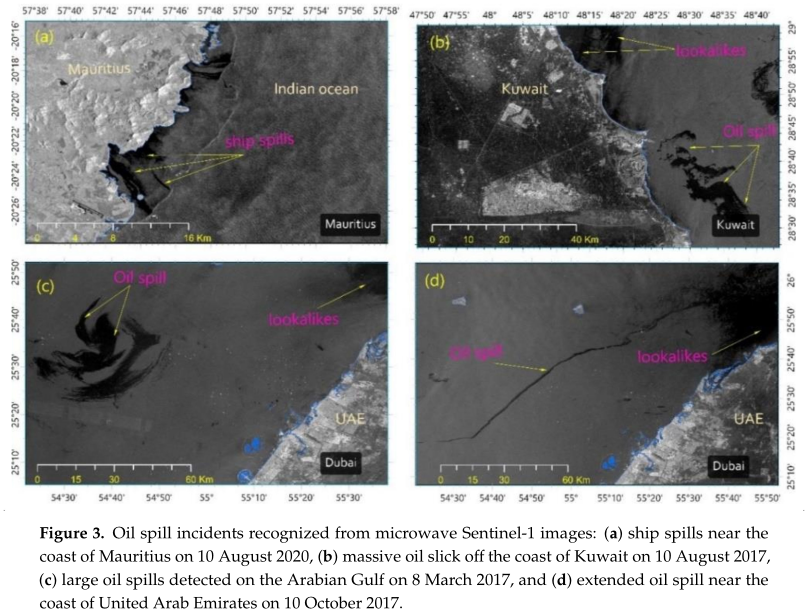
\includegraphics[scale=1.2]{img/section_02/caracteristicas_radar_01.png}
      \caption{Imágenes de radar}
      \label{fig:optical_features_01}
  \end{figure}
\end{frame}

\begin{frame}{Satélites de radar}
  \begin{figure}
      \centering
      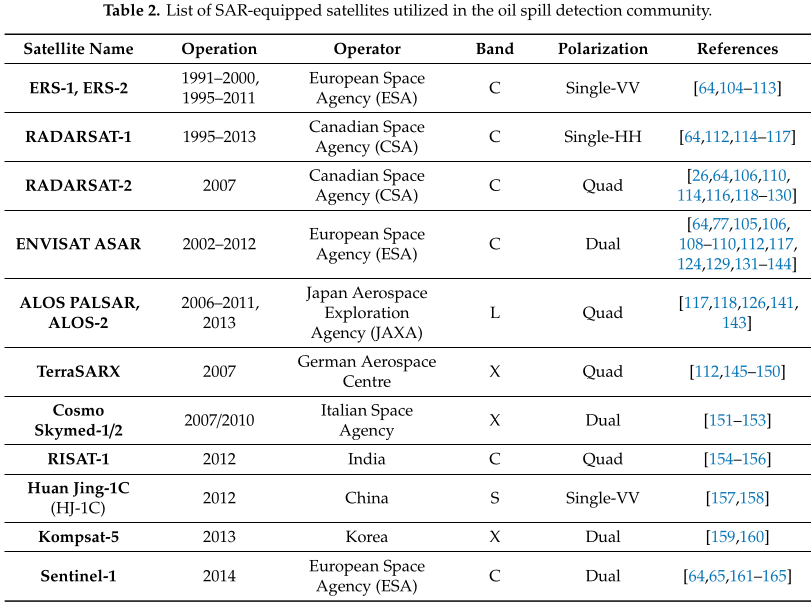
\includegraphics[scale=1.2]{img/section_02/caracteristicas_radar_02.png}
      \caption{Lista de satélites radar}
      \label{fig:optical_features_01}
  \end{figure}
\end{frame}

\begin{frame}{Extracción de características I}
  \begin{figure}
      \centering
      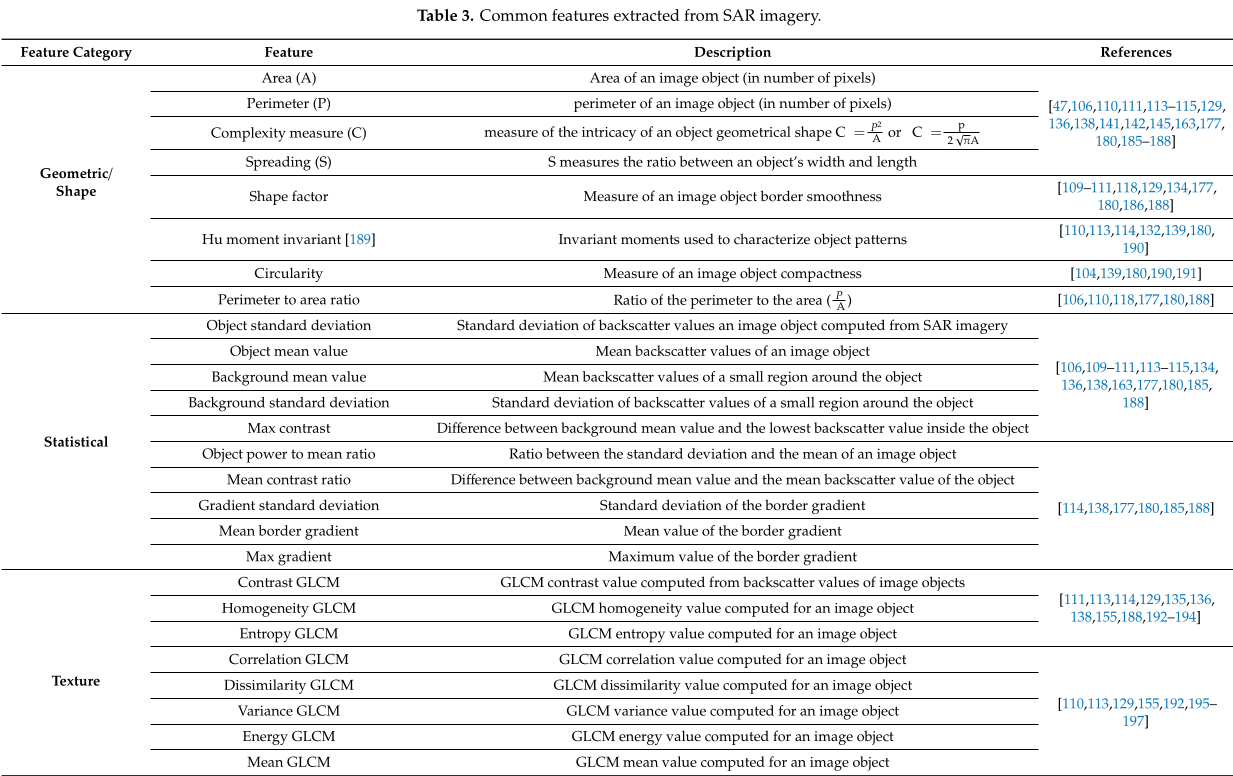
\includegraphics[scale=1.0]{img/section_02/tabla_caracteristicas_01.png}
      \caption{Características geométricas, estadísticas y de textura}
      \label{fig:optical_features_01}
  \end{figure}
\end{frame}

\begin{frame}{Extracción de características II}
  \begin{figure}
      \centering
      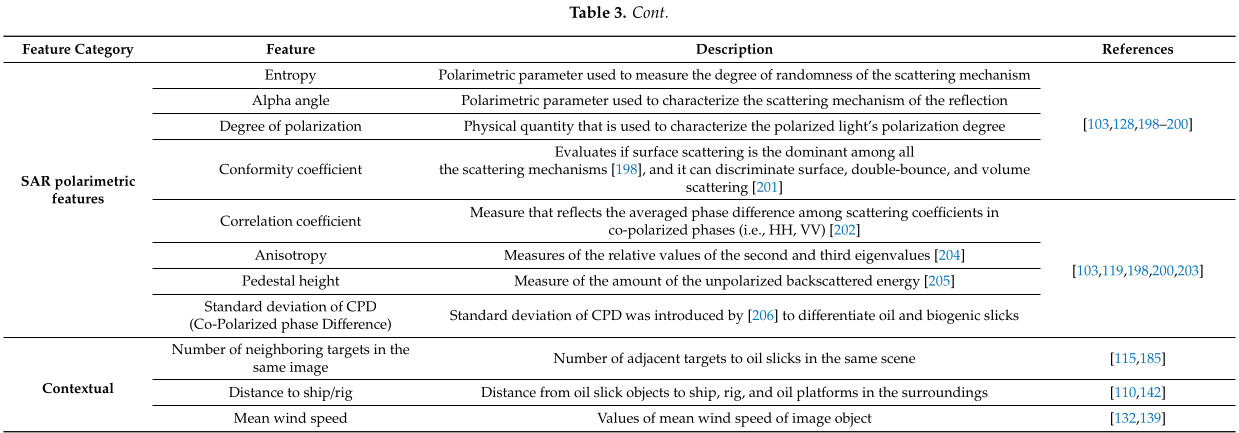
\includegraphics[scale=1.0]{img/section_02/tabla_caracteristicas_02.png}
      \caption{Características polarimétricas y contextuales}
      \label{fig:optical_features_01}
  \end{figure}
\end{frame}

\begin{frame}{Extracción de características III}
  \begin{figure}
      \centering
      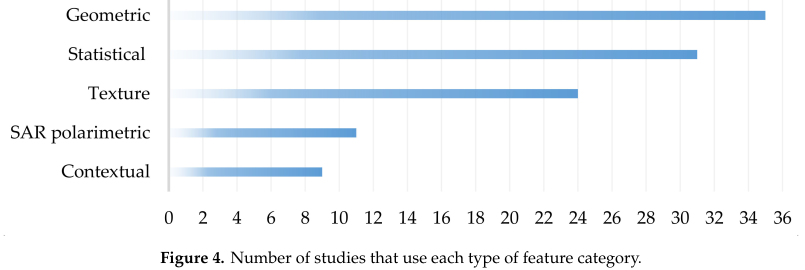
\includegraphics[scale=1.0]{img/section_02/tabla_caracteristicas_03.png}
      \caption{Cantidad de artículos por característica empleada}
      \label{fig:optical_features_01}
  \end{figure}
\end{frame}

\begin{frame}{Algoritmos clásicos de aprendizaje máquina}
    \begin{figure}
        \centering
        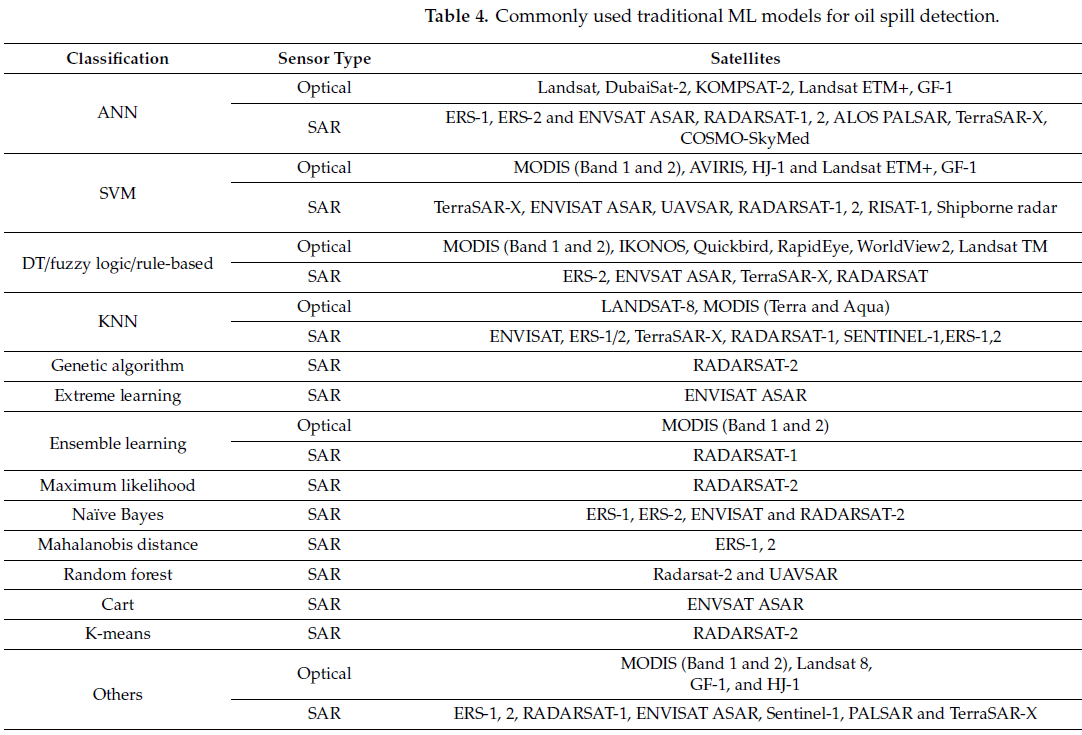
\includegraphics[scale=0.4]{img/section_02/oil_spill_detection_machine_learning.png}
        \caption{Classical Machine Learning}
        \label{fig:my_label}
    \end{figure}
\end{frame}

\begin{frame}{Algoritmos clásicos de aprendizaje máquina}
    \begin{figure}
        \centering
        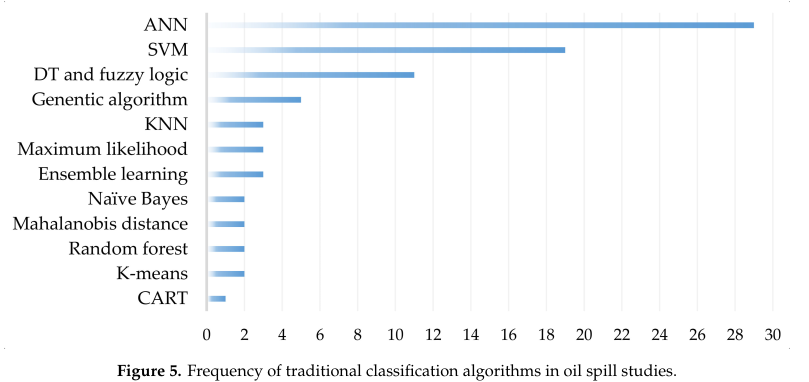
\includegraphics[scale=1.2]{img/section_02/frecuencias_machine_learning.png}
        \caption{Número de artículos por algoritmo}
        \label{fig:my_label}
    \end{figure}
\end{frame}

%\begin{frame}{Arquitectura de la CNN}
%    \begin{figure}
%        \centering
%        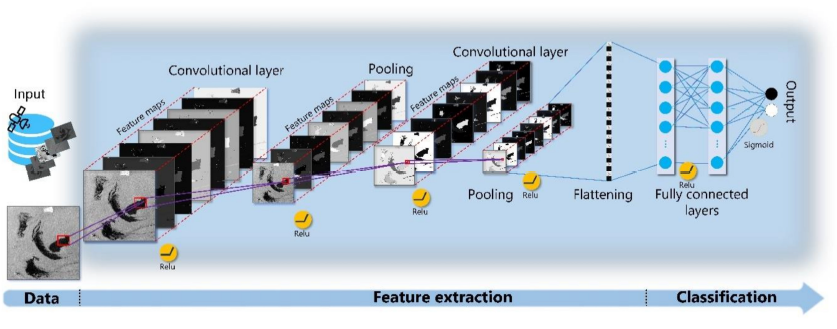
\includegraphics[scale=0.7]{img/section_02/oil_spill_detection_cnn_framework.png}
%        \caption{Convolutional Neural Network \cite{rs12203338}}
%        \label{fig:my_label}
%    \end{figure}
%\end{frame}

\begin{frame}{Algoritmos de aprendizaje profundo I}
    \begin{figure}
        \centering
        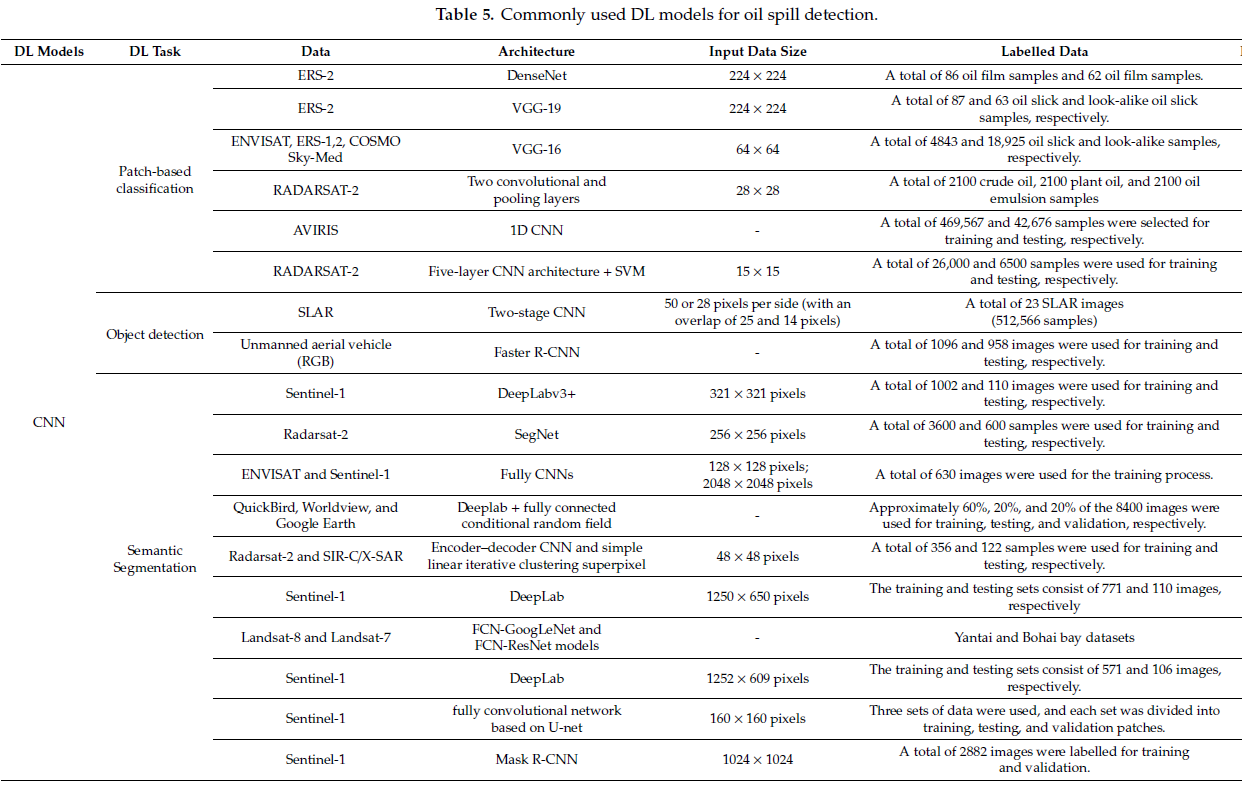
\includegraphics[scale=0.4]{img/section_02/oil_spill_detection_deep_learning.png}
        \caption{Deep Learning \cite{rs12203338}}
        \label{fig:my_label}
    \end{figure}
\end{frame}

\begin{frame}{Algoritmos de aprendizaje profundo II}
    \begin{figure}
        \centering
        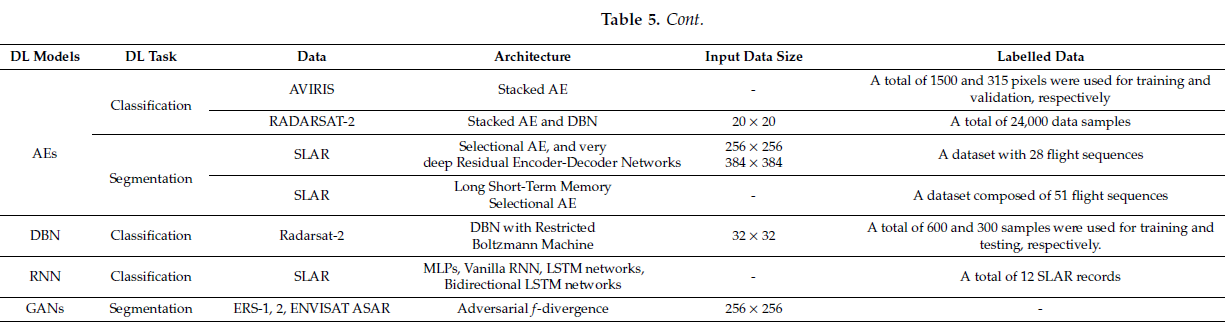
\includegraphics[scale=0.5]{img/section_02/oil_spill_detection_deep_learning2.png}
        \caption{Deep Learning \cite{rs12203338}}
        \label{fig:my_label}
    \end{figure}
\end{frame}


